\documentclass{article}

\usepackage{graphicx} % for images
\usepackage{amsmath} % for math
\usepackage{amssymb} % for \mathbb
\usepackage{siunitx} % for \SI, \num
\usepackage{hyperref} % for \url{}

% This stuff is for figures
\usepackage{float}
\DeclareGraphicsExtensions{.pdf, .png, .jpg}

% coloring of links for PDF format
\hypersetup{
    colorlinks=true,
    urlcolor=blue,
    linkcolor=blue
}

% \c command redefinition (for monospaced font)
\renewcommand{\c}[1]{\texttt{#1}}
% \today command re-definition
% https://tex.stackexchange.com/questions/112932/today-month-as-text
\renewcommand{\today}{\ifnum\number\day<10 0\fi \number\day \space%
\ifcase \month \or January\or February\or March\or April\or May%
\or June\or July\or August\or September\or October\or November\or December\fi\space%
\number \year} 

\begin{document}
\begin{titlepage}
	\centering
	\includegraphics[width=0.25\textwidth]{Images/247px-CSU-Longbeach_seal}\par\vspace{1cm}
	{\scshape\Large California State University, Long Beach \par}
	\vspace{1cm}
	{\scshape\Large Cecs 347\par}
	\vspace{1.5cm}
	{\huge\bfseries Project 1\par}
	\vspace{2cm}
    {\Large\itshape Rodrigo Becerril Ferreyra\par}
    {\itshape\Large Student ID 017584071 \par}
	\vfill
    A project that uses the ARM Cortex-M4 microcontroller to
    drive a car.

	\vfill

% Bottom of the page
	{\large \today\par}
\end{titlepage}

\section{Introduction}
The purpose of this project is to combine many different concepts
learned throughout the course so far: hardware PWM, PLL, and
DC motors. The requirement was to build a robot car that
could move at various different speeds, and move forwards and
backwards. My specific car has four wheels and four motors, so
I required double the amount of batteries.

\section{Operation}
My program operates as follows: first, all the required
clocks and registers are initialized once. This sets the
microcontroller up to its default running conditions (in this
case, forward operation at 30\% speed, with a green light).
After initialization, nothing else happens until an interrupt
is detected (the two on-board pushbuttons both trigger an
interrupt). If the left button is pressed, the speed of the
car cycles as follows:
\begin{equation*}
    30\% \rightarrow 60\% \rightarrow 80\% \rightarrow 98\% \rightarrow 0\%.
\end{equation*} The speed moves to the right every time the left
button is pressed (0\% loops back to 30\%). When the right button
is pressed, the car switches directions.

Here is a link to the operation of the car: \url{https://youtu.be/z8ZxZ9zTwM4}.

\section{Theory}
The microcontroller uses PWM (pulse-width modulation) to control
the speed of the car. PWM is a technique in where a signal
is repeatedly switched on and off to control the average power
delivered to a load. In this case, the load is a motor: if the
driving PWM signal is using a 30\% duty cycle, the motor will
only spin at 30\% its angular speed.

This project also uses PLL (phase-locked loop). The PLL module
in the microcontroller allows the system clock of \SI{16}{\mega\hertz}
to be increased up to \SI{80}{\mega\hertz}. For this project,
I am using a clock speed of \SI{50}{\mega\hertz}.
\pagebreak
\section{Hardware Design}
Figure \ref{fig:schematic diagram}
is a schematic diagram of my project. As noted in my video, I
am using 8 AA batteries, making my power source \SI{12}{\volt}.
Figure \ref{fig:3d pic} is an image of the physical car.

\begin{figure}[H]
    \centering
    \includegraphics[width=\textwidth]{Images/schemeit-project.pdf}
    \caption{Schematic Diagram of system.}
    \label{fig:schematic diagram}
\end{figure}
\begin{figure}[H]
    \centering
    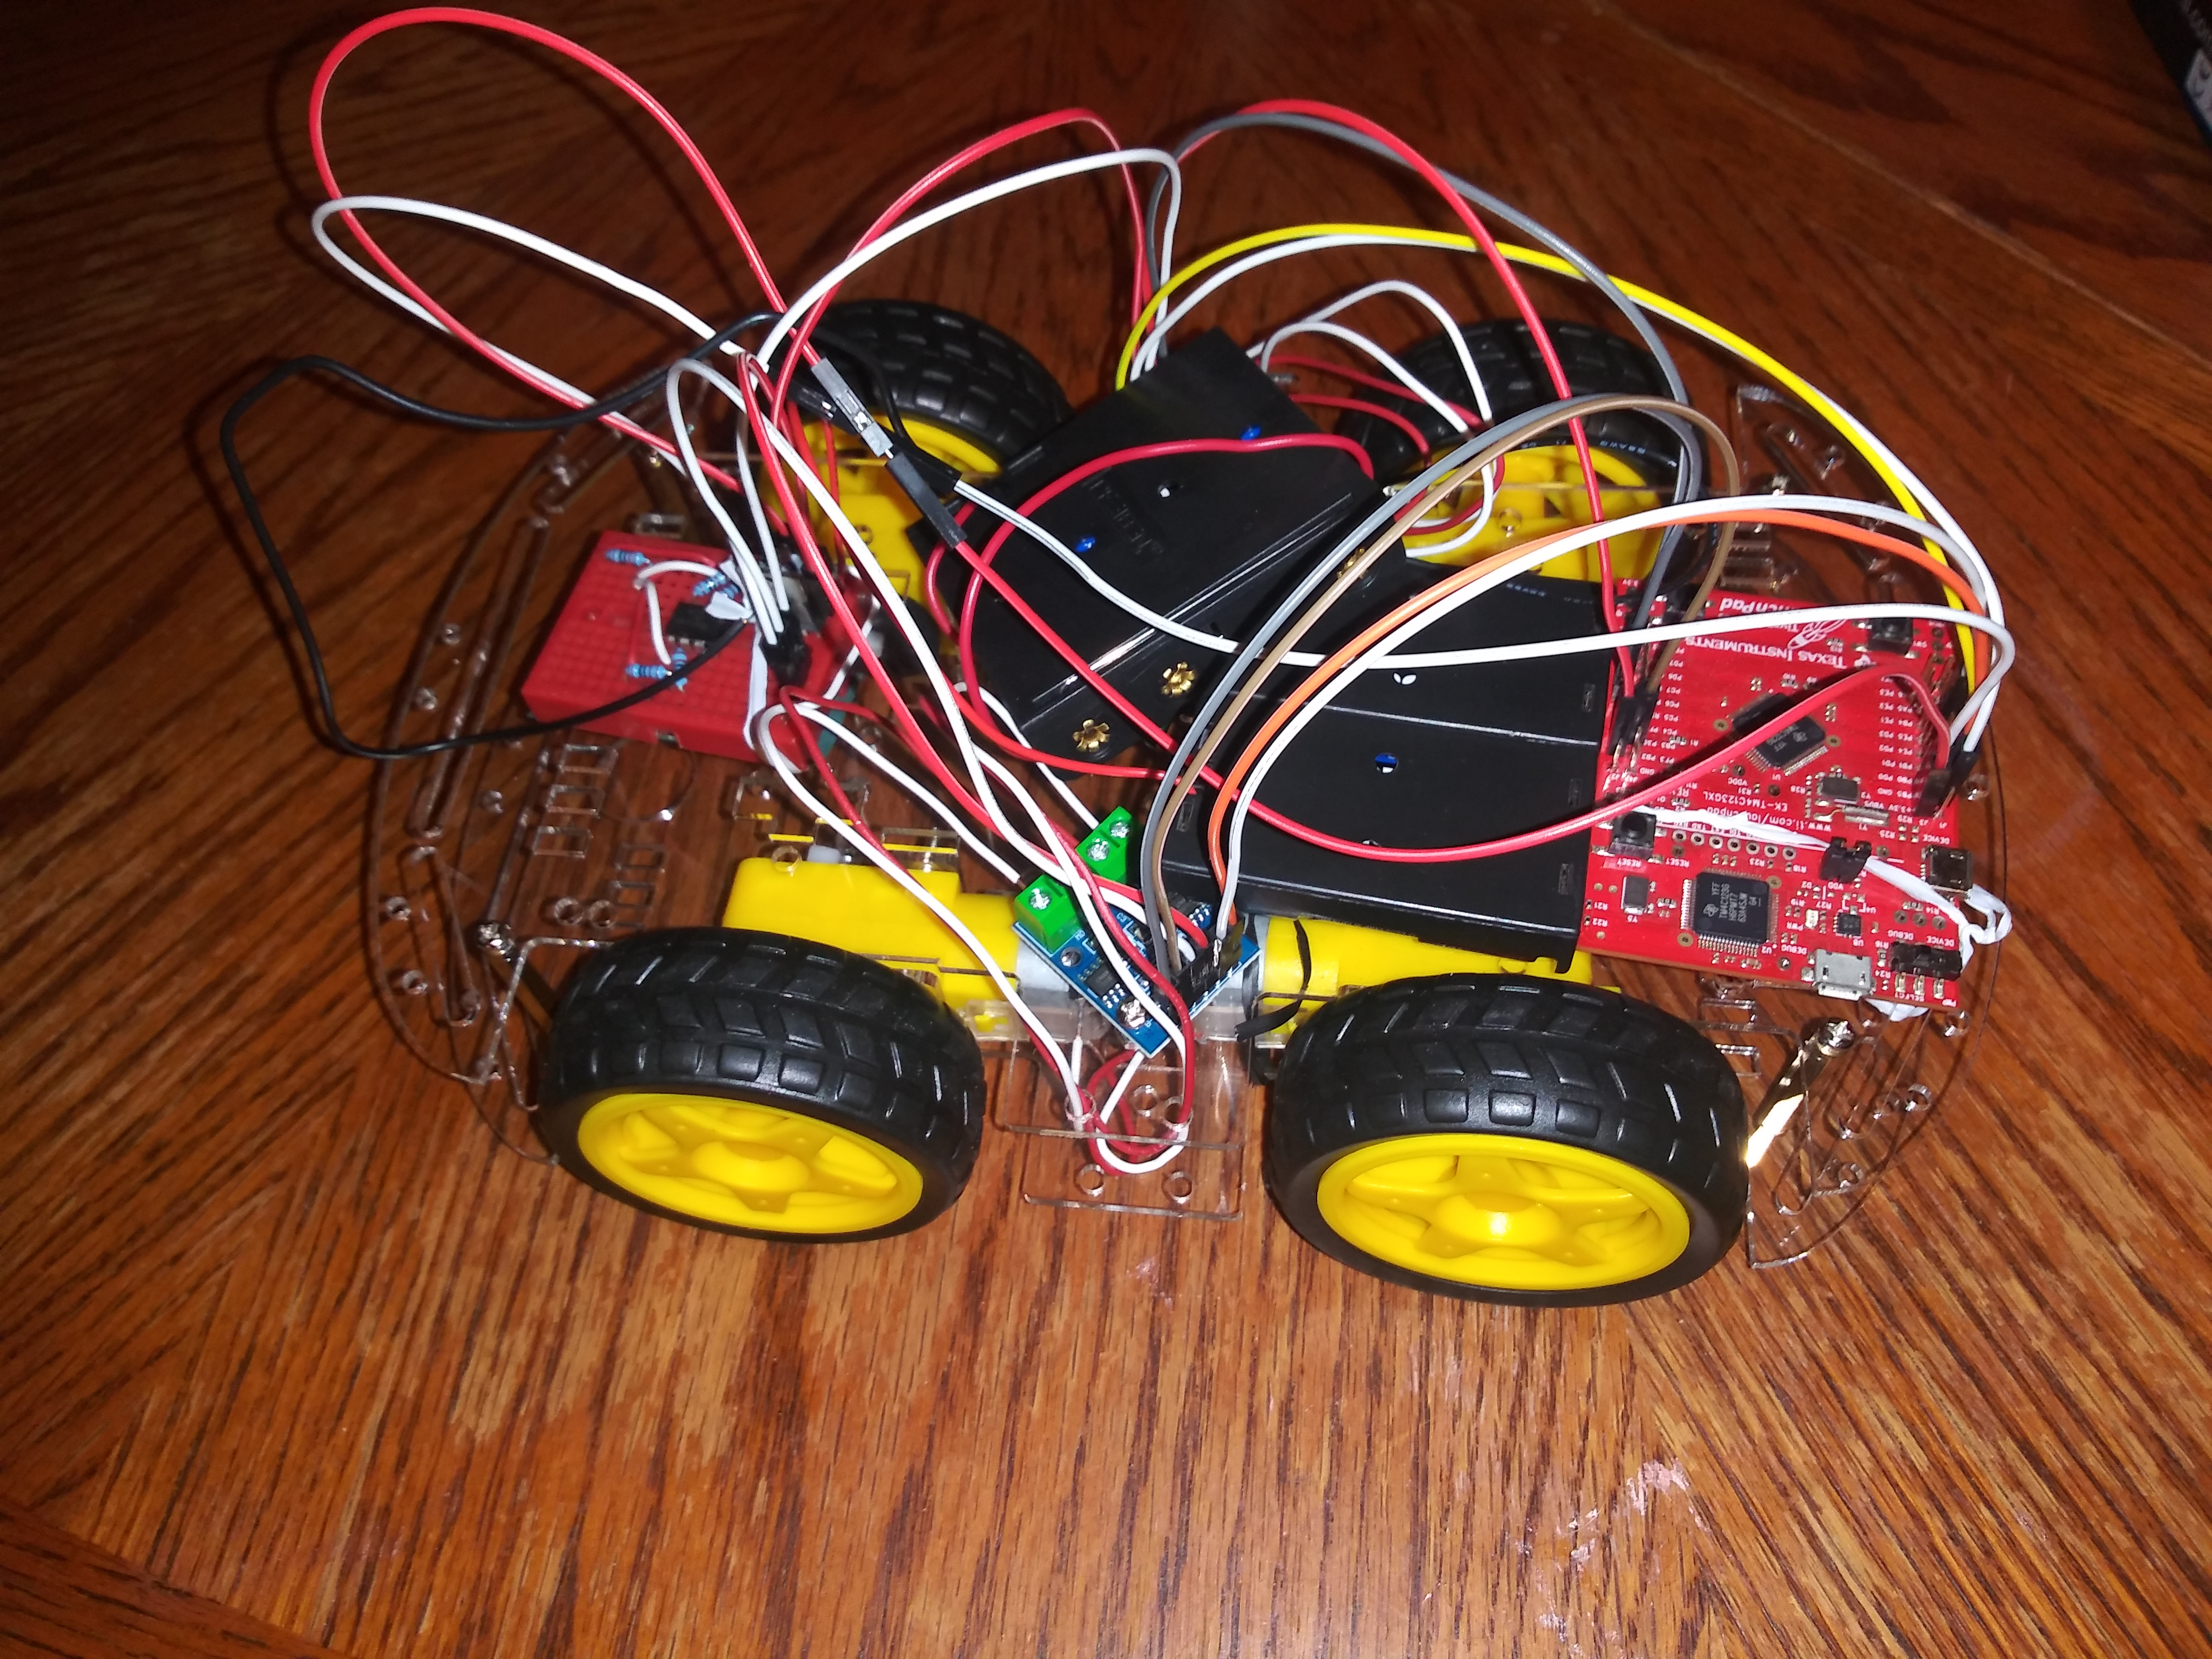
\includegraphics[width=\textwidth]{Images/20210305_223202.jpg}
    \caption{Picture of system.}
    \label{fig:3d pic}
\end{figure}

\section{Software Design}
I decided to put all the logic in the interrupt handler, to
make things simple. Originally, I was having issues, because
when the car was in the 30\% setting in the forward direction,
if the user switched the direction, the wheels would spin at
70\% speed. I managed to fix this, however.

\section{Conclusion}
Overall, I learned a lot from this project. I learned how many
different elements (such as PLL and PWM) can come together to
create one coherent system. I also learned the particulars in
setting up each element, what registers are involved, and
what can and cannot be done and in what order.

\end{document}
